%% fig_propagation.tex   (generated by make_frontier.py; do not edit by hand)
%% Propagation of algebraicity along a compact Shimura curve under the Lefschetz standard conjecture for the total space.
\documentclass[tikz,border=8pt]{standalone}
\usepackage{amsmath,amssymb}
\usetikzlibrary{arrows.meta,calc,decorations.pathreplacing}
%% palette.tex -- shared colour definitions for the figures
\definecolor{PInk}{RGB}{26,32,44}
\definecolor{PBlue}{RGB}{37,82,139}
\definecolor{PTeal}{RGB}{23,127,125}
\definecolor{POchre}{RGB}{193,138,44}
\definecolor{PClay}{RGB}{178,74,58}
\definecolor{PSlate}{RGB}{108,122,137}
\definecolor{PViolet}{RGB}{110,86,150}
\definecolor{WBlue}{RGB}{223,234,246}
\definecolor{WTeal}{RGB}{220,238,236}
\definecolor{WOchre}{RGB}{250,240,218}
\definecolor{WClay}{RGB}{247,229,224}
\definecolor{WSlate}{RGB}{238,241,244}
\definecolor{PMag}{RGB}{158,58,110}
\definecolor{PGrass}{RGB}{62,124,66}
\definecolor{PAmber}{RGB}{214,112,38}
\definecolor{PIndigo}{RGB}{58,64,140}
\definecolor{PRule}{RGB}{176,186,197}

%% shared macros so the standalone figures match the paper
\providecommand{\QQ}{\mathbb{Q}}
\providecommand{\ZZ}{\mathbb{Z}}
\providecommand{\RR}{\mathbb{R}}
\providecommand{\CC}{\mathbb{C}}
\providecommand{\PP}{\mathbb{P}}
\providecommand{\Kx}{K^{\times}}
\providecommand{\HW}{W}
\providecommand{\Nm}{\mathrm{N}}
\providecommand{\Hdg}{\mathrm{Hdg}}
\providecommand{\NS}{\mathrm{NS}}
\providecommand{\cA}{\mathcal{A}}
\providecommand{\cD}{\mathcal{D}}
\providecommand{\cF}{\mathcal{F}}
\providecommand{\cP}{\mathcal{P}}
\providecommand{\cO}{\mathcal{O}}
\providecommand{\cQ}{\mathcal{Q}}
\providecommand{\bbar}[1]{\overline{#1}}
\providecommand{\ch}{\operatorname{ch}}
\providecommand{\End}{\mathrm{End}}

\newcommand{\hcimp}{\,\textcolor{PIndigo}{\tiny$\Leftarrow\mathbf{HC}$}}
\begin{document}
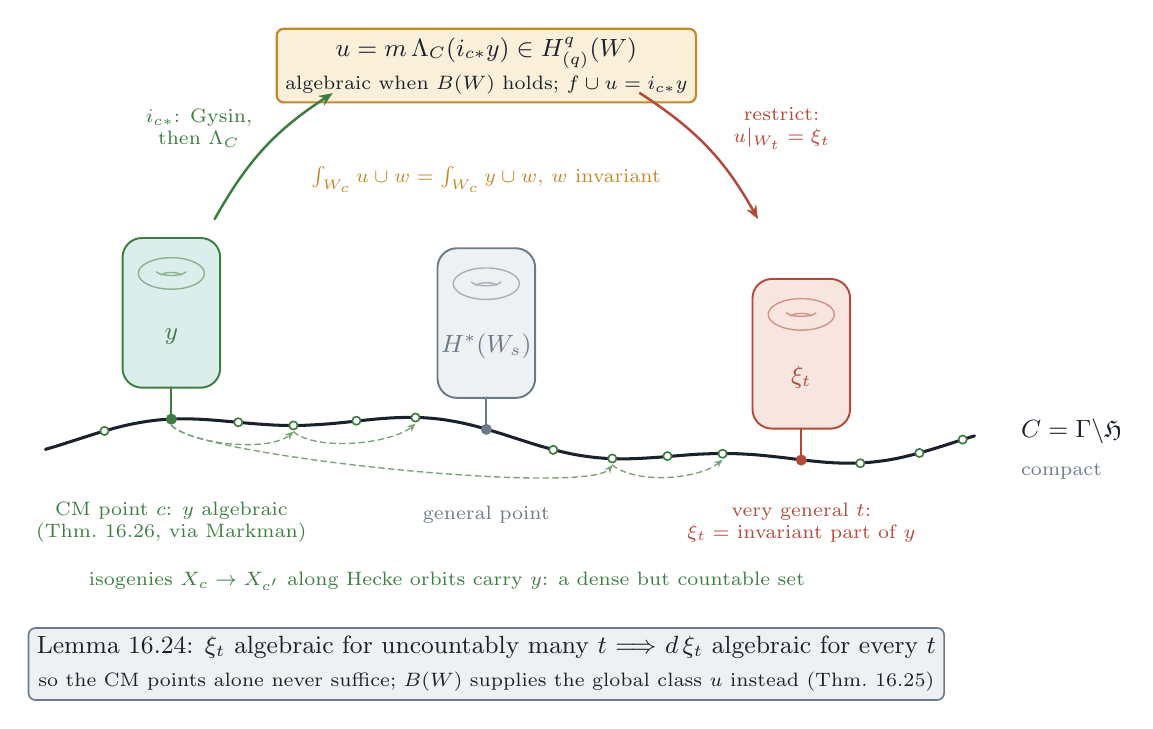
\begin{tikzpicture}[x=1cm,y=1cm,line join=round,line cap=round,
  font=\small,text=PInk]
  \draw[PInk,line width=1.1pt] (-0.40,-0.124) -- (-0.30,-0.095) -- (-0.20,-0.064) -- (-0.10,-0.032) -- (0.00,0.000) -- (0.10,0.032) -- (0.20,0.064) -- (0.30,0.095) -- (0.40,0.124) -- (0.50,0.151) -- (0.60,0.176) -- (0.70,0.198) -- (0.80,0.217) -- (0.90,0.233) -- (1.00,0.246) -- (1.10,0.255) -- (1.20,0.261) -- (1.30,0.264) -- (1.40,0.264) -- (1.50,0.261) -- (1.60,0.257) -- (1.70,0.250) -- (1.80,0.242) -- (1.90,0.233) -- (2.00,0.224) -- (2.10,0.215) -- (2.20,0.206) -- (2.30,0.198) -- (2.40,0.191) -- (2.50,0.185) -- (2.60,0.181) -- (2.70,0.180) -- (2.80,0.180) -- (2.90,0.182) -- (3.00,0.187) -- (3.10,0.193) -- (3.20,0.200) -- (3.30,0.209) -- (3.40,0.219) -- (3.50,0.230) -- (3.60,0.241) -- (3.70,0.251) -- (3.80,0.261) -- (3.90,0.269) -- (4.00,0.276) -- (4.10,0.280) -- (4.20,0.282) -- (4.30,0.282) -- (4.40,0.278) -- (4.50,0.271) -- (4.60,0.261) -- (4.70,0.247) -- (4.80,0.230) -- (4.90,0.210) -- (5.00,0.187) -- (5.10,0.161) -- (5.20,0.133) -- (5.30,0.103) -- (5.40,0.072) -- (5.50,0.040) -- (5.60,0.008) -- (5.70,-0.024) -- (5.80,-0.056) -- (5.90,-0.086) -- (6.00,-0.114) -- (6.10,-0.140) -- (6.20,-0.164) -- (6.30,-0.185) -- (6.40,-0.203) -- (6.50,-0.217) -- (6.60,-0.229) -- (6.70,-0.237) -- (6.80,-0.242) -- (6.90,-0.244) -- (7.00,-0.244) -- (7.10,-0.241) -- (7.20,-0.236) -- (7.30,-0.230) -- (7.40,-0.223) -- (7.50,-0.215) -- (7.60,-0.207) -- (7.70,-0.199) -- (7.80,-0.191) -- (7.90,-0.185) -- (8.00,-0.181) -- (8.10,-0.177) -- (8.20,-0.176) -- (8.30,-0.177) -- (8.40,-0.180) -- (8.50,-0.185) -- (8.60,-0.191) -- (8.70,-0.200) -- (8.80,-0.210) -- (8.90,-0.221) -- (9.00,-0.232) -- (9.10,-0.245) -- (9.20,-0.256) -- (9.30,-0.268) -- (9.40,-0.278) -- (9.50,-0.287) -- (9.60,-0.294) -- (9.70,-0.298) -- (9.80,-0.300) -- (9.90,-0.298) -- (10.00,-0.294) -- (10.10,-0.286) -- (10.20,-0.274) -- (10.30,-0.260) -- (10.40,-0.242) -- (10.50,-0.220) -- (10.60,-0.196) -- (10.70,-0.170) -- (10.80,-0.141) -- (10.90,-0.111) -- (11.00,-0.080) -- (11.10,-0.048) -- (11.20,-0.015) -- (11.30,0.016) -- (11.40,0.047);
  \node[text=PInk,inner sep=1pt,align=center,font=\small,anchor=west] at (11.95,0.10) {$C=\Gamma\backslash\mathfrak{H}$};
  \node[text=PSlate,inner sep=1pt,align=center,font=\scriptsize,anchor=west] at (11.95,-0.40) {compact};
  \draw[PGrass,fill=white,line width=0.6pt] (0.35,0.11) circle (1.5pt);
  \draw[PGrass,fill=white,line width=0.6pt] (1.20,0.26) circle (1.5pt);
  \draw[PGrass,fill=white,line width=0.6pt] (2.05,0.22) circle (1.5pt);
  \draw[PGrass,fill=white,line width=0.6pt] (2.75,0.18) circle (1.5pt);
  \draw[PGrass,fill=white,line width=0.6pt] (3.55,0.24) circle (1.5pt);
  \draw[PGrass,fill=white,line width=0.6pt] (4.30,0.28) circle (1.5pt);
  \draw[PGrass,fill=white,line width=0.6pt] (6.05,-0.13) circle (1.5pt);
  \draw[PGrass,fill=white,line width=0.6pt] (6.80,-0.24) circle (1.5pt);
  \draw[PGrass,fill=white,line width=0.6pt] (7.50,-0.21) circle (1.5pt);
  \draw[PGrass,fill=white,line width=0.6pt] (8.20,-0.18) circle (1.5pt);
  \draw[PGrass,fill=white,line width=0.6pt] (9.95,-0.30) circle (1.5pt);
  \draw[PGrass,fill=white,line width=0.6pt] (10.70,-0.17) circle (1.5pt);
  \draw[PGrass,fill=white,line width=0.6pt] (11.25,0.00) circle (1.5pt);
  \draw[PGrass!70,line width=0.5pt,dash pattern=on 2pt off 1.5pt,-{Stealth[length=3pt,width=2.5pt]}] (1.20,0.181) .. controls (1.50,-0.073) and (2.45,-0.155) .. (2.75,0.100);
  \draw[PGrass!70,line width=0.5pt,dash pattern=on 2pt off 1.5pt,-{Stealth[length=3pt,width=2.5pt]}] (2.75,0.100) .. controls (3.05,-0.155) and (4.00,-0.052) .. (4.30,0.202);
  \draw[PGrass!70,line width=0.5pt,dash pattern=on 2pt off 1.5pt,-{Stealth[length=3pt,width=2.5pt]}] (1.20,0.181) .. controls (1.50,-0.215) and (6.50,-0.718) .. (6.80,-0.322);
  \draw[PGrass!70,line width=0.5pt,dash pattern=on 2pt off 1.5pt,-{Stealth[length=3pt,width=2.5pt]}] (6.80,-0.322) .. controls (7.10,-0.571) and (7.90,-0.505) .. (8.20,-0.256);
  \node[text=PGrass,inner sep=1pt,align=center,font=\scriptsize] at (4.70,-1.80) {isogenies $X_{c}\to X_{c'}$ along Hecke orbits carry $y$: a dense but countable set};
  \draw[PGrass,fill=WTeal,line width=0.7pt,rounded corners=7pt] (0.58,0.66) rectangle (1.82,2.56);
  \draw[PGrass!60,line width=0.5pt] (1.20,2.11) ellipse (0.42 and 0.20);
  \draw[PGrass!60,line width=0.5pt] (1.01,2.13) arc (200:340:0.20 and 0.07);
  \draw[PGrass!60,line width=0.5pt] (1.07,2.09) arc (160:20:0.14 and 0.05);
  \draw[PGrass,line width=0.7pt] (1.20,0.261) -- (1.20,0.66);
  \fill[PGrass] (1.20,0.26) circle (2.0pt);
  \node[text=PGrass,inner sep=1pt,align=center,font=\small] at (1.20,1.31) {$y$};
  \draw[PSlate,fill=WSlate,line width=0.7pt,rounded corners=7pt] (4.58,0.53) rectangle (5.82,2.43);
  \draw[PSlate!60,line width=0.5pt] (5.20,1.98) ellipse (0.42 and 0.20);
  \draw[PSlate!60,line width=0.5pt] (5.01,2.00) arc (200:340:0.20 and 0.07);
  \draw[PSlate!60,line width=0.5pt] (5.07,1.96) arc (160:20:0.14 and 0.05);
  \draw[PSlate,line width=0.7pt] (5.20,0.133) -- (5.20,0.53);
  \fill[PSlate] (5.20,0.13) circle (2.0pt);
  \node[text=PSlate,inner sep=1pt,align=center,font=\small] at (5.20,1.18) {$H^{*}(W_{s})$};
  \draw[PClay,fill=WClay,line width=0.7pt,rounded corners=7pt] (8.58,0.14) rectangle (9.82,2.04);
  \draw[PClay!60,line width=0.5pt] (9.20,1.59) ellipse (0.42 and 0.20);
  \draw[PClay!60,line width=0.5pt] (9.01,1.61) arc (200:340:0.20 and 0.07);
  \draw[PClay!60,line width=0.5pt] (9.07,1.57) arc (160:20:0.14 and 0.05);
  \draw[PClay,line width=0.7pt] (9.20,-0.256) -- (9.20,0.14);
  \fill[PClay] (9.20,-0.26) circle (2.0pt);
  \node[text=PClay,inner sep=1pt,align=center,font=\small] at (9.20,0.79) {$\xi_{t}$};
  \node[text=PGrass,inner sep=1pt,align=center,font=\scriptsize] at (1.20,-1.05) {CM point $c$: $y$ algebraic\\(Thm.~16.26, via Markman)};
  \node[text=PSlate,inner sep=1pt,align=center,font=\scriptsize] at (5.20,-0.95) {general point};
  \node[text=PClay,inner sep=1pt,align=center,font=\scriptsize] at (9.20,-1.05) {very general $t$:\\$\xi_{t}=$ invariant part of $y$};
  \node[draw=POchre,fill=WOchre,rounded corners=2.5pt,inner sep=3pt,line width=0.80pt,align=center] at (5.20,4.75) {$u=m\,\Lambda_{C}(i_{c*}y)\in H^{q}_{(q)}(W)$\\[1pt]{\scriptsize algebraic when $B(W)$ holds; $f\cup u=i_{c*}y$}};
  \draw[PGrass,line width=0.90pt,-{Stealth[length=5pt,width=4pt]},bend left=14] (1.75,2.80) to (3.25,4.40);
  \draw[PClay,line width=0.90pt,-{Stealth[length=5pt,width=4pt]},bend left=14] (7.15,4.40) to (8.65,2.80);
  \node[text=PGrass,inner sep=1pt,align=center,font=\scriptsize] at (1.55,3.95) {$i_{c*}$: Gysin,\\then $\Lambda_{C}$};
  \node[text=PClay,inner sep=1pt,align=center,font=\scriptsize] at (8.95,3.95) {restrict:\\$u|_{W_{t}}=\xi_{t}$};
  \node[text=POchre,inner sep=1pt,align=center,font=\scriptsize] at (5.20,3.30) {$\int_{W_{c}}u\cup w=\int_{W_{c}}y\cup w$, $w$ invariant};
  \node[draw=PSlate,fill=WSlate,rounded corners=2.5pt,inner sep=3pt,line width=0.60pt,align=center] at (5.20,-2.85) {Lemma~16.24: $\xi_{t}$ algebraic for uncountably many $t$ $\Longrightarrow$ $d\,\xi_{t}$ algebraic for every $t$\\[1pt]{\scriptsize so the CM points alone never suffice; $B(W)$ supplies the global class $u$ instead (Thm.~16.25)}};
\end{tikzpicture}
\end{document}
